\chapter[Bending light to see into space]{Bending light to see into space\footnote{Initial lab written by Brent Barker. Home measurement setup, photos, and text provided by Chris Varney.}}

%todo feedback from 2019-fall:
% - uncertainty calculation was one step too much for many students. either remove or explicitly make it easy (=STDEV, or just do range of measurements)
% - logistics, mini-lecture, and queue instructions took 30 minutes
% - in step 4, give example table of observations
% - the 2 focal length measurements seemed redundant
% - lab was too long, most students did not get to making the telescope, but those who did thought it was really cool. formula constructing was out of reach for all.
% - students really wanted to know why light was refracting, not just that it was

Optical telescopes are one way that astronomers use to better observe the cosmos. In this lab, you will build up your understanding about how telescopes help us do this.

\section{Learning Goals}

\begin{itemize}
	\item Learn how light behaves when traveling between mediums.
	
	\item Create an image with a lens.
	
	\item Configure a refracting telescope and explain how it helps for observing the sky.
\end{itemize}

\section{Equipment needed}

\begin{itemize}
	\item Some sort of clear container with parallel sides that you can fill with water (e.g. Tupperware, fish tank)
	
	\item Two transparent hollow cylindrical containers (e.g. drinking glass, Nalgene bottle, Mason jar) of different diameters
	
	\item A small bright disperse light source (e.g. cell phone light, pen flashlight, NOT a laser pointer)
	
	\item A cardboard or similar box that you can cut a small slit into so that you only let a thin beam of light pass through it
	
	\item Something to measure distances with (e.g. meter stick, measuring tape, standard-sized objects you can look up the dimensions for like coins, credit cards, paper. You can even use an online ruler on your phone, e.g. \url{https://www.piliapp.com/actual-size/cm-ruler/})
\end{itemize}


%\section{But first! Observing with Stone Edge Observatory}
%
%Throughout the quarter, you will be taking data (images) with a robotic telescope that is located in Sonoma, California. This week, you will select a target and queue some images to be taken, at \url{queue.stoneedgeobservatory.com}. Please choose from one of the targets in Table\ \ref{lt:tab:targets}. The camera is a monochrome camera, broadly sensitive to all visible wavelengths ($\sim 400$--$700\:$nm). For now, let's collect light in all of those wavelengths by selecting the ``Clear'' filter, as well as leaving ``Dark'' checked.
%
%\renewcommand{\arraystretch}{1.2}
%
%\begin{table}
%	\begin{tabular}{p{0.6in}p{.8in}p{.9in}p{0.6in}p{0.9in}p{2in}}
%		target & RA & Dec & V-band & Suggested & Notes \\
%		& (hh mm ss) & ($\pm$ dd mm ss) & magnitude & exposure time (s) & \\ \hline
%		51 Pegasi & 22 57 27.9804 & +20 46 07.7822 & 5.46 & 15 & first Main Sequence star found to host an exoplanet \\
%		Altair & 19 50 46.9986 & +08 52 05.9563 & 0.76 & 5 & rapidly rotating star \\
%		
%		Betelgeuse & 05 55 10.3054 & +07 24 25.4304 & 0.42 & 5 & red supergiant star and one of the largest stars visible with the naked eye \\
%
%		Deneb & 20 41 25.91514 & +45 16 49.2197 & 1.25 & 10 & forms the Summer Triangle with Altair and Vega  \\
%	
%		Kelt-9 & 20 31 26.3534 & +39 56 19.7652 & 7.56 & 30 & hosts the hottest known gas giant exoplanet \\
%	
%		Epsilon Eridani & 03 32 55.8450  & -09 27 29.7312 & 3.73 & 15 & one of the nearest Sun-like stars with a planet and very young \\
%	
%		KIC 8462852 (aka Tabby's Star) & 20 06 15.4527 & +44 27 24.7914 & 12.01 & 90 & has very irregular changes in brightness (ask Prof. Fabrycky about what causes the dips!) \\
%	
%		Mira & 02 19 20.7921 & -02 58 39.4956 & 6.53 & 25 & variable binary system with a red giant and a white dwarf \\
%	
%		Polaris & 02 31 49.0946 & +89 15 50.7923 & 2.02 & 10 & lines up almost exactly with Earth's rotational axis to the north and is often called the North Star \\
%	
%		Sirius & 06 45 08.9173 & -16 42 58.0171 & -1.46 & 2 & brightest star in the sky \\
%	
%		UY Scuti & 18 27 36.5286 & -12 27 58.8933 & 11.20 & 90 & largest known star by radius \\
%	
%		Vega & 18 36 56.3364 & +38 47 01.2802 & 0.03 & 5 & one of the most well studied stars in the sky and has been used as a reference for calibrating photometric brightness scale for stars
%
%	\end{tabular}
%	\caption{List of targets for you to choose from.}\label{lt:tab:targets}
%\end{table}
%
%So that the queue is not overwhelmed, please limit your group's observations to one queue submission per student per week.

\section{Team roles}

\textbf{Decide on roles} for each group member. The available roles are:

\begin{itemize}
	\item Facilitator: ensures time and group focus are efficiently used
	\item Scribe: ensures work is recorded
	\item Technician: oversees apparatus assembly, usage
	\item Skeptic: ensures group is questioning itself
\end{itemize}

these roles can (will?) rotate each lab, and you will report at the end of the lab report on how it went for each role. If you have fewer than 4 people in your group, then some members will be holding more than one role.

\section{How do we use materials to bend light?}

We use lenses all the time to shape the path that light takes, either with eyeglasses or with optical telescopes. These activities are intended to help you understand how we use materials to bend light.

\subsection{Observing light refraction at home}

\begin{steps}

	\item You need an object that will refract the light. Find some sort of square or rectangular clear container (rounded edges are fine) and fill it with water. Small Tupperware is perfect for this.
	
	\item We need to create a beam of parallel light. Find something like a cardboard box (anything that will not let any light through and that nobody will mind if you cut chunks out of it). In the middle of one edge, cut a thin ($\sim{}1$ mm thick) slice 7--10 centimeters tall (we can cut it a little further later if we need). If you are clever about it, you can find a way to make this “wall” stand up on its own. Figure \ref{lt:fig:slit} shows the one Chris made out of a box from a microwave dinner. They stuck a single staple in the bottom corner that you can see to hold everything together so that it would hold itself upright.

\begin{figure}
	\centering
	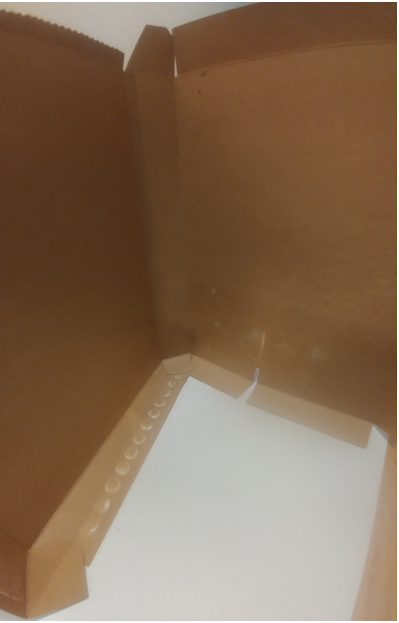
\includegraphics[width=0.6\textwidth]{lens-telescope/cardboard-slit.png}
	\caption{Thin slit cut into a cardboard box.}\label{lt:fig:slit}
\end{figure}

	\item Set your container on a sheet of paper and set it just beyond the slit. Set it up so that the light in incident to your container at an angle. A correct setup might look like Figure\ \ref{lt:fig:rect}.

\begin{figure}
	\centering
	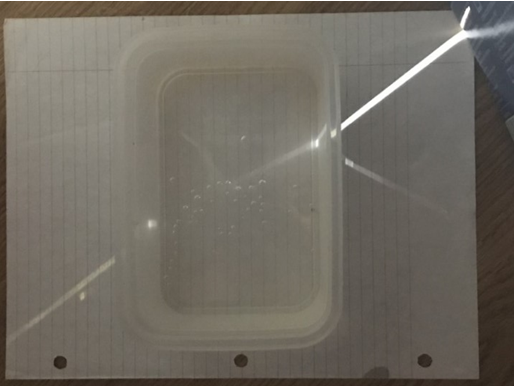
\includegraphics[width=0.6\textwidth]{lens-telescope/rectangle-refract.png}
	\caption{A ray of light enters one side of the water-filled container and exits the other side.}\label{lt:fig:rect}
\end{figure}

	Note that to get such a clear beam Chris had to tilt their light source slightly downward. They also needed to build their slit a little taller than they originally had made it. Try to find something that works for you. \textbf{Take a picture of your setup to include in your report.}

	\item Play with the angle at which the beam strikes the prism and observe what happens to its direction as it enters the prism (ignore the reflections or transmission through the other side, for now). How does the path of the laser beam change when it enters the prism? \textbf{Record your observations. Be specific about any patterns you notice.}

%	\item Find the laser and a trapezoidal prism in your kit. Set the prism on a white sheet of paper and adjust the laser so that it is shining into the prism from the side. Play with the angle at which the beam strikes the prism and observe what happens to its direction as it enters the prism (ignore the reflections or transmission through the other side, for now). How does the path of the laser beam change when it enters the prism? \textbf{Record your observations. Be specific about any patterns you notice.}
\end{steps}

\subsection{Careful observation with a simulated prism}

\begin{steps}
	\item It's hard to see the light in the prism, so let's use a simulation. Go to \url{https://phet.colorado.edu/en/simulation/bending-light} and select the play button to launch the simulation. Select the leftmost ``Intro'' box. This is a side view of the interface between two materials, currently air on the top half of the screen and water on the bottom. A laser is positioned above the interface.
	
	\item Play with the controls on this screen until you have an idea of how to move the laser, turn it on and off, and adjust the materials on the top and bottom. To reset the simulation, select the orange circular button on the lower right.
	
	\item Observe what happens to the laser beam when you change the a) angle, b) type of material on top and bottom, and c) indices of refraction. In each case, does the beam get deflected from its original straight-line path more, less, or the same amount? \textbf{Record your observations for your lab report in a table format.}

	\item Open the second screen at the bottom of the sim. Lenses are wider in the middle and thinner at the top and bottom, and we can model this with a circular prism. Drag a circle up and shine a ray through it. Set the laser to output several parallel rays and aim it so they hit the middle of the circle. \textbf{Record your observations of what the rays do when the exit the other side of the prism.}
	
%	\item Go back to your physical ray box and optics set. Adjust the ray box to emit 5 parallel rays. From the Pasco Optics Set, set up the convex lens (the one that is thinner on the ends and thicker in the middle) so that the rays are hitting it from the side. Notice where the rays go after they go through the lens. \textbf{Record your observations.}
\end{steps}

This setup of parallel rays is convenient for seeing precisely what the lens does. It also happens to be the situation when we observe things that are very far away compared to length scales of the lens. Consider two stakes driven into the ground next to each other, both perpendicular to the ground (and thus pointing directly at the center of the Earth). Since the Earth is a sphere, those stakes can't actually be both pointing directly toward the center of the Earth and also parallel to each other. For the former to be true, they must be angled slightly away from each other. But since the distance between them is so short compared to the distance away from the Earth's center, they are effectively parallel. \textit{This is the same with light arriving from distant objects like stars.}

\subsection{Imaging with a real lens}

\textbf{Goal:} Use a real lens to create an image, and calculate the focal length of the lens.

\begin{steps}

	\item Fill one of your cylindrical containers with water. Note that it needs to be as smooth and cylindrical as possible – tapered or textured edges will distort the image and affect your results. Place it about 30 cm away from a wall or some sort of screen that you can project an image onto. Move your small light source to be several container radii away from the container, on the other side from the wall/screen. Shine your small light source through the container “lens” so that the light should shine through it onto the wall/screen behind it. Move the container back and forth until you see a clear image on the screen. You should notice a thin vertical line of light that comes into focus if you hold the light at a specific distance from the lens. The point where this line is the thinnest is the point at which it is focused. \textbf{Draw a sketch of your setup, labeling the parts. Take a picture of your setup and of the image, if possible.}
%	\item For spherically symmetric lenses (or, in our case, a cylindrically symmetric lens), the focal length $f$ is easily calculated from the radius of curvature $R$ by
%\begin{equation}
%f = 2 R \,.
%\end{equation}
%	Make your measurement and record your result, with your estimate of uncertainty (for example, measure several times, then record your average value and also calculate the standard deviation of those values.\footnote{See the uncertainty appendix or visit \url{https://researchbasics.education.uconn.edu/calculatingmeanstandarddev/} for guidance on calculating these.}

%	\item Let's try putting some parallel rays from a distant object on a lens and see what happens where those rays intersect. Take one of the round lenses that are mounted in a black plastic frame and shine those parallel rays from the light box on it to find the distance where the rays intersect with each other. Hold a sheet of paper or hand in the path of the rays so you can see them.
	
%	\item Select a distant bright object with sharply contrasting edges. A good choice is the florescent ceiling lights in the hallway outside the lab. Hold the lens between the object and a white sheet of paper (or the floor if you are using the hallway ceiling lights). The white sheet of paper should be placed about the same distance away as the intersection distance from the previous step. \textbf{Record your observations.}
\end{steps}

If the object (light source) is a long distance away from the lens, compared to the distance from the lens to the image, then this intersection distance is called the focal length of the lens. The focal length is a property of the lens, based on its material and curvature. If an object is a long distance away compared to the focal length, then its image is formed at the focal length (if the object is closer, the image is formed further away than the focal length).

This principle works in reverse too --- if an object is placed at the focal length of the lens, the rays come out parallel on the other side. The image is effectively formed an infinite distance away.

\begin{steps}
	\item Design and conduct an experiment to measure the focal length of the lens you just used. Decide as a group how to measure, and how to estimate an uncertainty for your measurement. See Appendix\ \ref{cha:uncertainty} for detailed information about estimating uncertainty. \textbf{Record a sketch of your setup, a description of your procedure for gathering and analyzing your data, and the data itself, including your value of focal length with its uncertainty.}

%	\item Compare: how does this focal length compare to the focal length that is printed on the lens holder? See Appendix\ \ref{unc:sec:comparing} for how to compare two values, taking into account their uncertainties. \textbf{Record this comparison calculation and what you conclude about how close they are. Is the printed value correct?}
\end{steps}

This lens setup is great for producing images, for example to record onto photographic film or a digital camera's image sensor. It's less good for looking through the lens to magnify and gather more light the way we want to with a telescope. For that, we'll need at least two lenses.

\section{Your first telescope}

Telescopes come in many different configurations. Here you'll construct one that is simple by comparison, a refracting telescope, using just 2 lenses.

\begin{steps}
	\item Here's the principle for building this telescope: the image created by the first lens, called the objective lens, is the object for the second lens, which is called the eyepiece lens. The thing we are wanting to look at (the object for the objective lens) is far away. We want the image created by the eyepiece lens to be an infinite distance away on the near side (just trust me on this). \textbf{Given these design goals and the information about lenses above, where should the two lenses be positioned with respect to each other? Sketch your proposal, labeling each lens and drawing the focal lengths of each lens.}
	
	\item Acquire a second "lens" (cylindrical container filled with water), one with a different radius than the first one.
	
	\item Find the focal length of this lens the same way you found the length of other one.
	
	\item Construct your telescope by positioning the two lens on your surface according to your design.
	
	\item Test your telescope. Look at a distant (across the room) object through it. If you don't get a sharp image of it by looking through the eyepiece lens, iterate on your design until you get it.
	
	\item Find the magnification of your telescope. Hint: if you have two identical objects, how close does one need to be to look the same size/distance as the one you see through the telescope? Experimentally determine this magnification factor (1 is no magnification, 2 means it looks twice as close, 0.5 means that it looks twice as far away, etc), and estimate the uncertainty of your magnification. \textbf{Record this.}
	
	\item Magnification should be related to the properties of the two lenses. Make up a formula that relates the focal lengths of your lenses to the magnification of your telescope. You may need to switch the lenses around or use different ones to test your formula. \textbf{Record this.}
\end{steps}

\section{Report checklist and grading}

Each item below is worth 10 points. See Appendix\ \ref{cha:lab-report-format} for guidance on writing the report and formatting tables and graphs.

\begin{enumerate}
	
	\item Picture of setup and detailed observations from Steps 3--4.
	
	\item Sketch and picture of your setup and the image formed by your lens in Step 9.
	
	\item Detailed observations from Steps 7--8.
	
	\item Sketch and picture of your setup and procedure for finding the focal length in Step 10, as well as value, with uncertainty, of the focal length.
	
	\item Detailed sketch of your working telescope design, from Steps 11--15.
	
	\item Experimental determination of the magnification of your telescope, with uncertainty.
	
	\item Formula relating the focal lengths to the magnification.
	
	\item Discuss the findings and reflect deeply on the quality and importance of the findings. This can be both in the frame of a scientist conducting the experiment (``What did the experiment tell us about the world?'') and in the frame of a student (``What skills or mindsets did I learn?'').
	
	\item A 100--200 word reflection on group dynamics and feedback on the lab manual. Address the following topics: who did what in the lab, how did you work together, what successes and challenges in group functioning did you have, and what would you keep and change about the lab write-up?
	
	\item Write a paragraph reporting back from each of the four roles: facilitator, scribe, technician, skeptic. Where did you see each function happening during this lab, and where did you see gaps?
\end{enumerate}


%\begin{itemize}
%	\item Detailed observations from Steps 1--8.
%	
%	\item Sketch of your setup and procedure for finding the focal length in Step 9, as well as value, with uncertainty, of the focal length.
%	
%	\item Comparison of your measured focal length to the manufacturer's stated focal length, from Step 10.
%	
%	\item Detailed sketch of your working telescope design, from Steps 11--12.
%	
%	\item Experimental determination of the magnification of your telescope, with uncertainty.
%	
%	\item Formula relating the focal lengths to the magnification.
%	
%	\item Discuss the findings and reflect deeply on the quality and importance of the findings. This can be both in the frame of a scientist conducting the experiment (``What did the experiment tell us about the world?'') and in the frame of a student (``What skills or mindsets did I learn?'').
%	
%\end{itemize}